% Define the type of document we want to create
\documentclass[paper=a4,media/anfibrief,fromlogo=on]{scrlttr2}

% Packages
\usepackage[utf8]{inputenc}
\usepackage[htt]{hyphenat}
\usepackage[ngerman]{babel}
\usepackage{graphicx}
\usepackage{pdfpages}
\usepackage{eurosym}
\usepackage{graphics}
\usepackage{url} % especially useful for line breaks and online version
\PassOptionsToPackage{hyphens}{url} % avoids package loading clash with url and hyperref
\usepackage{hyperref}
\widowpenalty = 10000

\usepackage{fancyhdr}
\fancypagestyle{firststyle}
{
   \fancyhf{}
   \fancyfoot[C]{\tiny Source code available at \, \url{https://github.com/fsi-tue/anfibrief}\\ Latest version available at \, \url{https://teri.fsi.uni-tuebingen.de/anfibrief}\\ Revision: \gitCommit}
   \renewcommand{\headrulewidth}{0pt} % removes horizontal header line
}

% Metadata
\pdfinfo{
  /Author (Fachschaft Informatik)
  /Title  (Brief \studiengang)
  /Subject (\studiengang in Tuebingen)
  /Keywords (Erstsemester;FSI;WSI;Uni Tuebingen,Studienanfaenger;\studiengang)
}

% Beginning of the actual document
\begin{document}
  \date{\today}
  \setkomavar{subject}{\studiengang in T"ubingen }

  \begin{letter}
    {To all first-year students of\\
    \studiengang (\abschluss)\\
    \ifsommersemester
    summer semester \YEAR
    \fi
    \ifwintersemester
    winter semester \YEAR
    \fi
    }

    \opening{Dear newly-enrolled student,}

    % !TeX spellcheck = en_GB
\thispagestyle{firststyle}
We're really happy that you're starting your studies in \studiengang in Tübingen!
To help you get started, we want to provide you with some information to help you get through your first few weeks.

Who or what is this \glqq student council\grqq? We, the student council of computer science, are a group of students from the subjects computer science, bioinformatics, media computer science, medical informatics, and machine learning
who commit themselves to the students' interests. Our work includes, on one hand, the representation of students in university bodies, on the other hand, we try to facilitate the university lives of our fellow students (i.e. beginners care,
events, mentoring, and so on).

\ifmaster
    \ifml
We recommend participating in our beginners' events because the transition to master's studies or from another university respectively often proves to be difficult. This way you get a first look into everyday life in Tübingen.
    \fi
\fi
At our events, there will be many students in higher semesters who are eagerly waiting to answer all your questions. You can find an overview of our events on the following pages.

In case you have questions before or after our events, you can reach us by mail at \texttt{fsi\At fsi.uni-tuebingen.de}
On our home page
\url{https://www.fsi.uni-tuebingen.de} you can already find helpful information about your studies. If you're interested in collaborating with the student council, just come to one of our meetings! The current date will be published on our web page.

We're excited to meet you at our beginners events!\\
%\vfill
Your student council of computer science
\enlargethispage{3\baselineskip} % we dont want the last line(s) to be put on an extra page
\par\hfill{\footnotesize Editors: Mathis \& Clara}
\vfill

% \noindent\makebox[\textwidth][c]{%
% 	\setlength{\fboxrule}{4pt}
% 	\fcolorbox{green}{white}{
% 		\begin{minipage}[t]{
% 				\textwidth}
% 			If you aren't vaccinated yet, then you can get a vaccination in the special program of the university.\\
% 			More information can be found on \url{https://uni-tuebingen.de/universitaet/infos-zum-coronavirus/impfen} or \url{https://dranbleiben-bw.de}.
% \end{minipage}}}

    %\vfill
    %\input{src/ps_zulassung}
    \pagebreak
    \Fett{Your schedule for the first days}
    %\Fett{Euer Terminkalender für die ersten Tage}
    \enlargethispage{1ex}
    
% Roter Kasten mir Corona Disclaimer und anmeldung für events.
\setlength{\fboxrule}{4pt}
    \fcolorbox{red}{white}{
        \begin{minipage}[t]{\textwidth}
            \ifml
                \textbf{Attention!} The dates of these events may still change.
                Be sure to check \url{https://www.fsi.uni-tuebingen.de/du-bist-ersti}, we will publish the latest information there.\\\\
                    % HINWEIS ZUR ANMELDUNG - GILT IMMER - NICHT LÖSCHEN
                \textbf{Note:} \textbf{Please register for all events}, unless it is explicitly stated that no registration is necessary.
                Further details on the respective event and the registration can always be found on \url{https://eei.fsi.uni-tuebingen.de}.
                If you have registered for an event but will not be attending, please deregister again.
            \else
                \textbf{Achtung!} Die Termine der Erstiveranstaltungen könnten sich noch ändern.
                Schau auf jeden Fall auf \url{https://www.fsi.uni-tuebingen.de/du-bist-ersti} nach, dort werden wir die aktuellsten Daten veröffentlichen.\\\\
                    % HINWEIS ZUR ANMELDUNG - GILT IMMER - NICHT LÖSCHEN
                \textbf{Bitte melde dich zu allen Veranstaltungen an}, außer es steht explizit dabei, dass keine Anmeldung notwendig ist.
                Die Anmeldung ist in der Regel ab einer Woche vor der jeweiligen Veranstaltung möglich.\\
                Falls du dich zu einer Veranstaltung angemeldet hast und doch nicht kommen wirst, dann melde dich bitte auch wieder ab.
                Weitere Details und die Anmeldung zur jeweiligen Veranstaltung  findest du auch immer auf \url{https://eei.fsi.uni-tuebingen.de}.
            \fi
        \end{minipage}}
\begin{description}

% TODO für die Folgejahre nach WS23: alle Vorkurse mit TBA-Angaben wieder mit den herausgefundenen Daten einkommentieren :)

% Kogni Mathe Vorkurs
\ifkogwiss
    \ifmaster
        \item[\parbox{\linewidth}{Mathevorkurs-Master -- Mittwoch, 01. Oktober bis Donnerstag, 09. Oktober \YEAR,\\ 09:00--17:00 Uhr, Sand C214}]\ \vspace{.355\baselineskip} \\ % parbox and vspace since the line is too long
        %Heute beginnt der Vorbereitungskurs Mathematik speziell für Kognitionswissenschaftler:innen im Master.
        Es gibt einen Vorbereitungskurs Mathematik speziell für Kognitionswissenschaftler:innen im Master.
        Es ist zwar nicht Pflicht, daran teilzunehmen, aber sehr empfehlenswert. Nicht zuletzt lernt ihr hier erste Mitstudierende kennen! Der Vorkurs bietet euch eine Zusammenfassung des Mathestoffs, der im Bachelor Kognitionswissenschaft an der Uni Tübingen behandelt wird.
        \textbf{Wenn ihr euren Bachelor nicht an der Universität Tübingen oder in einem anderen Fach erworben habt, kann der Vorkurs für euch sinnvoll sein.} Falls ihr Quereinsteiger seid, werdet ihr dadurch an die in eurem Studium benötigten mathematischen Grundlagen herangeführt. Falls ihr bereits mathematisches Vorwissen mitbringt, ist der Kurs eine gute Gelegenheit, euer Wissen aufzufrischen.\\
        Es wäre super, wenn ihr euch mit einer kurzen Mail an \texttt{kogni-beratung@fsi.uni-tuebingen.de} anmelden würdet. Alle weiteren Infos erhaltet ihr dann per Mail.\\
        %Stattfinden wird der Vorkurs im ÜR 08 in der alten Physik, das ist die Gmelinstraße 6. Diese befindet sich an der Bushaltestelle Gmelinstraße, nördlich gegenüber von der Neuen Aula. Wenn ihr auf der Wilhelmstraße seid, geht rechts an der Neuen Aula vorbei, dort findet ihr die Alte Physik an der Ecke Gmelin- und Nauklerstraße, rechts von der Neuen Aula. Seid ihr auf der Hölderlinstraße, geht links dran vorbei und die Alte Physik ist auf der linken Straßenseite. Genaue Informationen bezüglich Treffpunkt am ersten Termin erhaltet ihr dann nochmal per Mail.
        %
        %\seticon{faBus}~\textbf{Bushaltestelle:} Gmelinstraße, Hölderlinstraße, Uni/Neue Aula
        \seticon{faBus}~\textbf{Bushaltestelle:} Sand Drosselweg (Linien 2 \& 6)
        %
    %\else
    \fi
\fi

\ifmaster
    \ifbinfo
        \item[Informatikvorkurs -- \bioinfoDatum~\YEAR]\ \\
        Es gibt einen Informatik-Vorkurs speziell für Bioinformatik-Studierende (Variante B) im Master. 
        Dieser Vorkurs wird dringend empfohlen, wenn du aus einem fachfremden Studiengang wie z.B. Biologie oder anderen Lebenswissenschaften kommst und nur wenig Erfahrung in der Informatik und der Programmierung (CLI, Java, Python, \LaTeX) hast. Der Vorkurs wird auf Englisch gehalten. \\
        \textbf{Anmeldeschluss:} \bioinfoAnmeldung\YEAR\\
        Anmeldung/Infos unter: \url{https://uni-tuebingen.de/de/215092}\\
        Kontakt: \texttt{\bioinfoKontakt}\\
        \seticon{faBus}~\textbf{Bushaltestelle:} Sand Drosselweg (Linien 2 \& 6)
    \fi
\fi

% Mathe-Vorkurs (nicht ML und nicht Kogni Master und nicht Lehramt Master)
\ifmaster
    \ifml %
    \else
        \ifkogwiss %
        \else
            \iflehramt %
            \else
                \item[Mathevorkurs -- \mathedatum~\YEAR]~\\
                Wenn du deinen Bachelor nicht in Tübingen oder in einem mathefremden Fach erworben hast, kann dieser Vorkurs für dich sehr sinnvoll sein. Auf unserer Website findest du ein Skript mit den Inhalten des Vorkurses. Damit solltest du einschätzen können, wie viel vom Stoff bereits bekannt ist und ob sich der Besuch des Vorkurses lohnt.\smallskip \\
                Der Vorkurs bietet dir eine Wiederholung des Schulstoffes und eine Einführung in die Uni-Mathematik. Zudem hast du die Möglichkeit, einige deiner neuen Mitstudierenden kennenzulernen und erste Lerngruppen zu bilden.

                \textbf{Anmeldeschluss:} \matheanmeldung\YEAR\\
                Anmeldung/Infos unter: \url{https://uni-tuebingen.de/de/91877}\\
                Kontakt: \texttt{\mathkontakt}
                \ifsommersemester
                    \\ \seticon{faBus}~\textbf{Bushaltestelle:} Sand Drosselweg (Linien 2 \& 6)
                \fi
            \fi
        \fi
    \fi
\fi

\ifbachelor
    \item[Mathevorkurs -- \mathedatum~\YEAR]~\\
    Von der Uni wird ein Vorbereitungskurs für Mathematik angeboten. Es ist zwar nicht Pflicht, daran teilzunehmen, aber es ist sehr empfehlenswert.
    Der Vorkurs bietet dir eine Wiederholung des Schulstoffes und eine Einführung in die Uni-Mathematik. Zudem hast du die Möglichkeit, einige deiner neuen Mitstudierenden kennenzulernen und erste Lerngruppen zu bilden.

    \textbf{Anmeldeschluss:} \matheanmeldung\YEAR\\
    Anmeldung/Infos unter: \url{https://uni-tuebingen.de/de/91877}\\
    Kontakt: \texttt{\mathkontakt}
    \ifsommersemester
        \\ \seticon{faBus}~\textbf{Bushaltestelle:} Sand Drosselweg (Linien 2 \& 6)
    \fi
\fi

%%%%%%%%%%%%%%%%%%%%%%%%%%%%%%%%%%%%%%%%%%%%%%%%%%%%%%%%%%%%%%%%%%%%%%%%%%%%
% Ab hier die FSI Events einfügen. Darüber sind der Mathe und Info vorkurs.

%Spieleabend 1
\ifml
    \item[Board Game Night 1 -- Wednesday, October 1st \YEAR, Sand]~\\%, 19:00, Sand]~\\
    We'd like to invite you to a board game night in relaxed atmosphere at the Sand.
    We'll provide some games as well as drinks and snacks (for a small donation).
    Even though our collection is growing steadily, we're more than happy if you bring along your own games!\\
    \seticon{faBus}~\textbf{bus stop:} Sand Drosselweg (bus lines 2 \& 6)
\else
    \item[Spieleabend 1 -- Mittwoch, 1. Oktober \YEAR, Sand]~\\%, 19:00 Uhr, Sand]~\\
    Wir möchten dich zu einem kleinen Analog-Spieleabend mit guter Gesellschaft und entspannter Atmosphäre auf dem Sand einladen.
    Für einige Spiele sowie Getränke und Knabberkram (gegen einen kleinen Obolus) sorgt die Fachschaft.
    Wir freuen uns natürlich sehr, wenn du auch eigene Spiele mitbringst, obwohl unsere Sammlung schon beachtlich ist!\\
    \seticon{faBus}~\textbf{Bushaltestelle:} Sand Drosselweg (Linien 2 \& 6)
\fi

%Flunkyball
\ifml
    \item[Flunkyball -- Tuesday, October 21th \YEAR, Sand]~\\
    Fancy a round of flunkyball? Come along, grab a bottle and have fun!
    Perfect opportunity to switch off and meet new people.
    Teams can be formed spontaneously and you can get beer from us for a small donation.\\
    \seticon{faBus}~\textbf{bus stop:} Sand Drosselweg (bus lines 2 \& 6)
\else
    \item[Flunkyball -- Dienstag, 21. Oktober \YEAR, Sand]~\\
    Lust auf 'ne Runde Flunkyball? Komm vorbei, schnapp dir 'ne Flasche und hab Spaß!
    Perfekte Gelegenheit, um abzuschalten und neue Leute kennenzulernen.
    Teams können spontan gebildet werden und Bier kannst du von uns gegen eine kleine Spende bekommen.\\
    \seticon{faBus}~\textbf{Bushaltestelle:} Sand Drosselweg (Linien 2 \& 6)
\fi

% Nur damit die Seite richtig gebrochen wird.
% TODO: Muss jedes jahr angepasst werden.
% \ifbinfo \ifmaster \pagebreak  \fi \fi

%Wanderung 1
\ifml
\item[Hike 1 -- Saturday, October 11th \YEAR, 10:30, on the Neckarinsel (Neckar Island)]~\\
On a leisurely hike you will get to know not only your fellow students,
but also a few lecturers and the worthwhile surroundings of Tübingen!
% The meeting point is at the Neckarbrücke \emph{in front of the} restaurant \glqq Neckarmüller\grqq.\\
The meeting point is on the Neckarinsel.\\
\seticon{faBus}~\textbf{bus stop:} Neckarbrücke (lines 1--22)
\else
\item[Wanderung 1 -- Samstag, 11. Oktober \YEAR, 10:30 Uhr, auf der Neckarinsel]~\\
Bei einer gemütlichen Wanderung lernt ihr neben euren Kommilitonen und Kommilitoninnen auch
noch ein paar Dozierende und die sehenswerte Tübinger Umgebung kennen!
% Der Treffpunkt ist bei der Neckarbrücke (\emph{vor} dem Gasthaus \glqq Neckarmüller\grqq).\\
Der Treffpunkt ist auf der Neckarinsel.\\
\seticon{faBus}~\textbf{Bushaltestelle:} Neckarbrücke (Linien 1--22)
\fi

% Nur damit die Seite richtig gebrochen wird.
% TODO: Muss jedes jahr angepasst werden.
\ifmaster \ifinfo \iflehramt \else \pagebreak \fi \fi \fi
\ifmaster \ifmedien \pagebreak \fi \fi
\ifmaster \ifmedinfo \pagebreak \fi \fi
\ifmaster \ifkogwiss \pagebreak \fi \fi

% Kneipentour 1 % TODO Uhrzeit
\ifml
    \item[Pub Crawl 1 -- Tuesday, October 7th \YEAR]~\\
    Tübingen is a town full of small pubs and bars that characterize the nightlife.
    To calm down from the stress of this information-filled day, we'd like to invite you to go bar-hopping with us.
    We'll divide up into small groups and visit the different bars in the historic town center.
    Please bring enough cash, most places we will visit don't accept cards (\emph{none whatsoever}).
\else
    \item[Kneipentour 1 -- Dienstag, 7. Oktober \YEAR]~\\
    Tübingen ist übersät mit kleinen Kneipen und Bars, die das Nachtleben maßgeblich bestimmen.
    Um den Stress der ersten Veranstaltungen etwas sacken zu lassen, laden wir dich zu einer ausgiebigen Kneipentour ein,
    bei der wir in Kleingruppen die verschiedenen Lokalitäten der Tübinger Altstadt besuchen.
    Bitte bringe genügend Bargeld mit, man kann in fast keiner der Tübinger Bars mit EC-Karte zahlen! -- Volksbanken und Sparkassen finden sich bei Bedarf in der Stadt.
\fi

% Nur damit die Seite richtig gebrochen wird.
% TODO: Muss jedes jahr angepasst werden.
\ifbachelor \pagebreak \fi

% Semestereröffnung
\ifml
    \vspace{-2.07182\baselineskip} \ \\ % to counteract the different spacing of the parbox in the line below. Remove this line if you remove the parbox and vspace in the line below
    \item[\parbox{\linewidth}{Semester Opening by Faculty -- Thursday, October TODO \YEAR, 16:15,\\ Audimax, Neue Aula}]\ \vspace{.355\baselineskip} \\ % parbox and vspace since the line is too long
    This department information event with presentation of all elective courses in the winter
    semester is especially useful if you are new to Tübingen and want to get a first impression
    of the professors and courses you will be dealing with in the future.\\
    \seticon{faBus}~\textbf{bus stop:} Uni/Neue Aula or Hölderlinstraße
\else
    \vspace{-2.07182\baselineskip} \ \\ % to counteract the different spacing of the parbox in the line below. Remove this line if you remove the parbox and vspace in the line below
    \item[\parbox{\linewidth}{Semestereröffnung Fachbereich -- Donnerstag, TODO. Oktober \YEAR, 16:15 Uhr,\\ Audimax, Neue Aula}]\ \vspace{.355\baselineskip} \\ % parbox and vspace since the line is too long
    Informationsveranstaltung des Fachbereichs mit Vorstellung aller
    Wahlveranstaltungen im Wintersemester.
    \ifbachelor
        Die Veranstaltung richtet sich vor allem an höhere Semester,
        wer als hochmotivierter Bachelor-Ersti Informationen sammeln will, darf natürlich dennoch vorbeischauen.
    \else
        Diese Veranstaltung ist besonders sinnvoll, wenn du neu nach Tübingen kommst um dir ein erstes Bild davon zu machen,
        mit welchen Professoren und Veranstaltungen du es zukünftig zu tun hast.
    \fi \\
    \seticon{faBus}~\textbf{Bushaltestelle:} Uni/Neue Aula oder Hölderlinstraße
\fi

%Spieleabend 2 %TODO time
\ifml
    \item[Board Game Night 2 -- Wednesday, October 15th \YEAR, Sand]~\\%, 19:00, Sand]~\\
    We'd like to invite you to a board game night in relaxed atmosphere at the Sand.
    We'll provide some games as well as drinks and snacks (for a small donation).
    Even though our collection is growing steadily, we're more than happy if you bring along your own games!\\
    \seticon{faBus}~\textbf{bus stop:} Sand Drosselweg (bus lines 2 \& 6)
\else
    \item[Spieleabend 2 -- Mittwoch, 15. Oktober \YEAR, Sand]~\\%, 19:00 Uhr, Sand]~\\
    Wir möchten dich zu einem kleinen Analog-Spieleabend mit guter Gesellschaft und entspannter Atmosphäre auf dem Sand einladen.
    Für einige Spiele sowie Getränke und Knabberkram (gegen einen kleinen Obolus) sorgt die Fachschaft.
    Wir freuen uns natürlich sehr, wenn du auch eigene Spiele mitbringst, obwohl unsere Sammlung schon beachtlich ist!\\
    \seticon{faBus}~\textbf{Bushaltestelle:} Sand Drosselweg (Linien 2 \& 6)
\fi

% Frühstück
\ifbachelor
    \item[Frühstück -- Freitag, 10. Oktober \YEAR, 10:00 Uhr, Mensa Morgenstelle]\ \\
    Wir laden dich an diesem Morgen zu einem gemütlichen Frühstück ein! Dabei erfährst du einiges über die Uni, die Fachschaft und was dich in den nächsten Monaten erwartet -- auch im Gespräch mit älteren Studierenden.
    Danach machen wir eine Führung über die Morgenstelle, damit du die wichtigsten Räume und Hörsäle kennenlernst.
    Wenn du Lust hast, kannst du anschließend ab 11:45 Uhr das Mensaessen ausprobieren.\\
    \seticon{faBus}~\textbf{Bushaltestelle:} BG Unfallklinik (Linien 5, 13, 14, 17, 18, 19, X15)
\fi

% %Mastercafé
% \ifmaster
%     \ifml
%         \item[Mastercafé -- Friday, October 11th \YEAR, 14:30]\ \\
%         At this informal meeting you will have the opportunity to get to know your fellow students and some of the lecturers over a coffee. And then there will be cake.\footnote{This is not a lie!}\\
%         % \seticon{faBus}~\textbf{bus stop:} route 3, "`Maria-von-Linden-Straße"' (signposted from there)
%         % \seticon{faBus}~\textbf{bus stop:} Sand Drosselweg (bus lines 2 \& 6)
%    \else
%         \item[Mastercafé -- Freitag, 11. Oktober \YEAR, 14:30 Uhr]\ \\
%         Bei diesem informellen Treffen hast du Gelegenheit, neue Master-Studierende aus deinem eigenen und auch aus anderen Studiengängen sowie einige der Dozierenden bei Kaffee kennenzulernen. Und dann gibt es Kuchen.\footnote{Das ist keine Lüge!}\\
%         % \seticon{faBus}~\textbf{Bushaltestelle:} Sand Drosselweg (Linien 2 \& 6)
%    \fi
% \fi

% Grillen 1
\ifml
    \item[BBQ 1 -- Friday, October 10th \YEAR, 18:30, in the garden of the Sand]~\\
    You're not in the mood for cooking this evening? Fear not!
    The student council invites you for a BBQ. Bring whatever you want to put on the grill,
    please also bring your own plates and cutlery. The garden has enough space for stuff like volleyball, football etc. as well.\\
    \seticon{faBus}~\textbf{bus stop:} Sand Drosselweg (bus lines 2 \& 6)
\else
    \item[Grillen 1 -- Freitag, 10. Oktober \YEAR, 18:30 Uhr, im Garten des Sandes]~\\
    Du hast keinen Bock auf Kochen? Dann bist du hier genau richtig! In geselliger Runde wird die Fachschaft mit dir grillen.
    Bring dazu mit, was auch immer du zum Grillen brauchst, ein großer Gasgrill wartet auf dich. Vergiss bitte auch nicht, dein eigenes Besteck und Geschirr einzupacken!\\
    Auf dem Sand ist es auch möglich Volleyball, Fußball, usw. zu spielen. Wir freuen uns auf dich!\\
    \seticon{faBus}~\textbf{Bushaltestelle:} Sand Drosselweg (Linien 2 \& 6)
\fi

% Erste Vorlesung
\ifbachelor
    \item[Erste Vorlesung -- Montag, 14. Oktober \YEAR, \ifwintersemester 8:00 Uhr, \else 10:00 Uhr, \fi Morgenstelle]~\\
    Deine erste Vorlesung beginnt um
    \ifwintersemester 8:00 Uhr -- Du hast „Mathematik für Informatik 1“  \fi
    \ifsommersemester 10:00 Uhr -- Du hast „Mathematik für Informatik 2“  \fi
    bei \Matheprof.
    Alles, was du heute (und in Zukunft) benötigst: persönlichen Wachmacher, einen Stift, einen Block und den Studierendenausweis.\\
    \seticon{faBus}~\textbf{Bushaltestelle:} BG Unfallklinik (Linien 5, 13, 14, 17, 18, 19, X15)
\fi

% Kneipentour 2 % TODO Uhrzeit
\ifml
\item[Pub Crawl 2 -- Tuesday, October 14th \YEAR]~\\
    Ready for round two? Join us for another pub crawl through Tübingen's best spots.
    We'll split into smaller groups again and visit the different bars in the historic town center.
    Please bring enough cash, most places we will visit don't accept cards (\emph{none whatsoever}).
\else
\item[Kneipentour 2 -- Dienstag, 14. Oktober \YEAR]~\\
    Bereit für Runde Zwei? Komm mit auf eine weitere Kneipentour durch die besten Kneipen Tübingens.
    Wir werden uns wieder in kleinere Gruppen aufteilen und die verschiedenen Bars in der Altstadt besuchen.
    Bitte bringe genügend Bargeld mit, man kann in fast keiner der Tübinger Bars mit EC-Karte zahlen! -- Volksbanken und Sparkassen finden sich bei Bedarf in der Stadt.
\fi

% Filmeabends % TODO date & time % TODO invite ML, movie language?
\ifml
    \item[TODO Movie Night -- Tuesday, October 15th \YEAR, 19:00, Sand]~\\%, 19:00, Sand]~\\
    % Falls im Wintersemester ein Filmeabend veranstaltet wird, sollte in der Einladung erwähnt werden, auf welcher
    % Sprache der Film gezeigt wird.
    In the evening, we're hosting a movie night, and we'd love for you to join us!
    It'll be a great way to unwind after your first days of student life.
    Bring your new friends and your favorite snacks, and let's go!
    Drinks will be provided for a small donation.\\
    \seticon{faBus}~\textbf{bus stop:} Sand Drosselweg (bus lines 2 \& 6)
\else
    \item[TODO Filmeabend -- Dienstag, 15. Oktober, 19:00 Uhr, Sand]~\\
    Am Abend veranstalten wir unseren Filmeabend und wir laden euch herzlich dazu ein!\\
    Schaut mit uns einen Film an und entspannt euch nach euren ersten Tagen im Studileben.
    Bringt eure neuen Freunde, Freundinnen und eure Lieblingssnacks mit und los geht's!\\
    Für Getränke ist gegen eine kleine Spende gesorgt.\\
    \seticon{faBus}~\textbf{Bushaltestelle:} Sand Drosselweg (Linien 2 \& 6)
\fi

% Nur damit die Seite richtig gebrochen wird.
% TODO: Muss jedes jahr angepasst werden.
\ifbachelor \pagebreak \fi
\ifmaster \ifinfo \iflehramt \else \pagebreak \fi \fi \fi
\ifmaster \ifmedien \pagebreak \fi \fi
\ifmaster \ifmedinfo \pagebreak \fi \fi
\ifmaster \ifkogwiss \pagebreak \fi \fi

% % Kastenlauf
% \ifml
% \item[Crate Run -- Wednesday, October 16th \YEAR, Rewe West]~\\
%     Please join us on our crate run.
%     Each team of two to four will have a crate (can be purchased on site).
%     The goal is to have emptied the crate at the finish line.
%     On your tour you will have to visit a few stops.
%     We don't force anyone to drink, you are also welcome to drink non-alcoholic beer, soft drinks, or whatever you like.
%     So if you're up for meeting new people, good vibes, and a little sporty drinking, feel free to drop by! \\
%     \seticon{faBus}~\textbf{bus stop:} Schleifmühleweg (bus lines 11 \& 12)
% \else
% \item[Kastenlauf -- Mittwoch, 16. Oktober \YEAR, Rewe Weststadt]~\\
%     Wir laden euch herzlich zu unserem Kastenlauf ein.
%     Jedes Zweier- bis Viererteam hat einen Kasten (kann vor Ort gekauft werden).
%     Das Ziel ist es, an der Ziellinie den Kasten leergetrunken zu haben.
%     Auf eurer Tour müsst ihr dabei verschiedene Stationen besuchen.
%     Unser Motto: Wer nicht wankt, der nicht gewinnt!\footnote{Wir zwingen niemanden zum Saufen, ihr dürft auch gerne alkoholfreies Bier, Softdrinks, etc. trinken.}
%     Wer also Lust hat auf neue Leute, gute Laune und ein wenig sportliches Trinken, kann gerne vorbeischauen! \\
%     \seticon{faBus}~\textbf{Bushaltestelle:} Schleifmühleweg (Linien 11 \& 12)
% \fi

% % Akademischer Spieleabend %TODO time
% \ifml
%     \item[Academic Game Night -- Thursday, October 17th \YEAR, Sand]~\\%, 19:00, Sand]~\\
%     This game night is a bit different. You can expect to find drinking games here,
%     but there are also non-alcoholic drinks for those who prefer to stick to water or soft drinks.\\
%     \seticon{faBus}~\textbf{bus stop:} Sand Drosselweg (bus lines 2 \& 6)
% \else
%     \item[Akademischer Spieleabend -- Donnerstag, 17. Oktober \YEAR, Sand]~\\%, 19:00 Uhr, Sand]~\\
%     Im Unterscheid zum "`normalen"' Spieleabend stehen hier vor allem Trinkspiele auf dem Programm.
%     Natürlich gibt es aber auch alkoholfreie Getränke.\\
%     \seticon{faBus}~\textbf{Bushaltestelle:} Sand Drosselweg (Linien 2 \& 6)
% \fi

% Nur damit die Seite richtig gebrochen wird.
% TODO: Muss jedes jahr angepasst werden.
% \ifmaster \ifbinfo \else \ifml \else \pagebreak \fi \fi \fi

% Grillen 2
\ifml
    \item[BBQ 2 -- Saturday, October 18th \YEAR, 18:30, in the garden of the Sand]~\\
    Because it's so nice, we'll have another barbecue!
    Bring whatever you'd like to grill, and don’t forget your own plates and cutlery!\\
    You can also play volleyball, football, and more in the garden. We’re looking forward to seeing you there!\\
    \seticon{faBus}~\textbf{bus stop:} Sand Drosselweg (bus lines 2 \& 6)
\else
    \item[Grillen 2 -- Samstag, 18. Oktober \YEAR, 18:30 Uhr, im Garten des Sandes]~\\
    Und weils so schön ist, grillen wir nochmal!
    Bring mit, was auch immer du grillen möchtest. Eigenes Besteck und Geschirr bitte nicht vergessen!\\
    Auf dem Sand ist es auch möglich Volleyball, Fußball, usw. zu spielen. Wir freuen uns auf dich!\\
    \seticon{faBus}~\textbf{Bushaltestelle:} Sand Drosselweg (Linien 2 \& 6)
\fi

% % Capture the Flag
% \ifml
%     \item[Capture the Flag -- Sunday, October 20th \YEAR, 14:00, Sand]~\\
%     We play a round of Capture the Flag together in real life.
%     A wonderful opportunity to test our teamwork skills and meet new friends (or enemies).\\
%     \seticon{faBus}~\textbf{bus stop:} Sand Drosselweg (bus lines 2 \& 6)
% \else
%     \item[Capture the Flag -- Sonntag, 20. Oktober \YEAR, 14:00 Uhr, Sand]~\\
%     Wir spielen gemeinsam eine Runde real-life Capture the Flag.
%     Eine wunderbare Gelegenheit, unsere Teamwork-Fähigkeiten zu testen und neue Freunde (oder Feinde) kennenzulernen.\\
%     \seticon{faBus}~\textbf{Bushaltestelle:} Sand Drosselweg (Linien 2 \& 6)
% \fi

%Wanderung 2
\ifml
    \item[Hike 2 -- Saturday, October 25th \YEAR, 10:30, on the Neckarinsel (Neckar Island)]~\\
    Time for another hike! Join us for a relaxing stroll through the beautiful Tübingen countryside.
    This is a great chance to enjoy nature, chat with fellow students, and maybe even meet some of your professors.
    % The meeting point is at the Neckarbrücke \emph{in front of the} restaurant \glqq Neckarmüller\grqq.\\
    The meeting point is on the Neckarinsel.\\
    \seticon{faBus}~\textbf{bus stop:} Neckarbrücke (lines 1--22)
\else
    \item[Wanderung 2 -- Samstag, 25. Oktober \YEAR, 10:30 Uhr, auf der Neckarinsel]~\\
    Zeit für eine weitere Wanderung! Komm mit auf einen entspannten Spaziergang durch die schöne Umgebung Tübingens.
    Bei einer gemütlichen Wanderung lernt ihr eure Kommilitonen und Kommilitoninnen
    und vielleicht auch ein paar Dozierende kennen!
    % Der Treffpunkt ist bei der Neckarbrücke (\emph{vor} dem Gasthaus \glqq Neckarmüller\grqq).\\
    Der Treffpunkt ist auf der Neckarinsel.\\
    \seticon{faBus}~\textbf{Bushaltestelle:} Neckarbrücke (Linien 1--22)
\fi

%Clubhausfest
\ifml
    \item[Clubhausfest -- Thursday, October 23th \YEAR, 21:00, Clubhaus]\ \\
    Every thursday during the lecture period, a different student body or group of students organizes the "`Clubhaus Fest"' in
    the Clubhaus, which locates directly opposite of the new auditorium. Today the attendance is particularly worthwhile, because
    the student councils of computer science, cognitive science, psychology, neurobiology and geography are hosting the event! \\
    No registration necessary.\\
    \seticon{faBus}~\textbf{bus stop:} Uni/Neue Aula or Hölderlinstraße
\else
    \item[Clubhausfest -- Donnerstag, 23. Oktober \YEAR, 21:00 Uhr, Clubhaus]\ \\
    Während der Vorlesungszeit richtet jeden Donnerstag eine andere Fachschaft oder studentische Gruppierung das Clubhausfest
    im Clubhaus, direkt gegenüber der Neuen Aula, aus. Heute lohnt sich der Besuch jedoch ganz besonders, denn die Fachschaften
    Informatik, Kogni, Psychologie, Neurobiologie und Geographie sind Gastgeber! % \\ % TODO line break wieder einfügen: Eigentlich wäre hier ein line break schöner, aber im WS24 würde dann eine einzelne Zeile auf die nächste Seite kommen
    Keine Anmeldung nötig.\\
    %Das anfängliche Chaos des Vorlesungsbeginns hat sich gelegt und auch an diesem Donnerstag findet das Clubhausfest statt.\\
    \seticon{faBus}~\textbf{Bushaltestelle:} Uni/Neue Aula oder Hölderlinstraße
\fi

% Nur damit die Seite richtig gebrochen wird.
% TODO: Muss jedes jahr angepasst werden.
% \ifml \pagebreak \fi

\ifml
   % TODO?
\else
   \item[Erstihütte -- Freitag, 07. November bis Sonntag, 09. November \YEAR]~\\
   Vom 01. bis 03. November fahren wir auf die Erstihütte in Dettingen.
   Euch erwartet ein geselliges Programm und ein entspanntes Miteinander.
   Weitere Informationen bezüglich Anmeldung folgen.
\fi

%Schnuppersitzung % TODO date & time
\ifkogwiss
    % \item[Schnuppersitzung der fsk -- TBA (reguläre Sitzungen: Donnerstags, 18:30, vor dem Kogni Zimmer), Sand]~\\%Donnerstag, 18. Mai \YEAR, 18:30 Uhr, Sand]~\\
    % Hoffentlich konnten wir mit unseren Veranstaltungen euer Interesse an Fachschaftsarbeit wecken.
    % Wir machen aber noch viel mehr als nur Ersti-Veranstaltungen, wir vertreten die Studierenden in Gremien,
    % sind Ansprechpartner, stellen Infrastruktur und Tools bereit und vieles mehr.
    % Komm doch einfach mal zu unserer Schnuppersitzung
    % \footnote{Natürlich freuen wir uns auch sehr, wenn du sogar schon vor der Schnuppersitzung zu regulären Sitzungen kommst :)}
    % und schau ob es dir gefällt!\\
    % Keine Anmeldung nötig.\\
    % \seticon{faBus}~\textbf{Bushaltestelle:} Sand Drosselweg (Linien 2 \& 6)
\else
    \ifml
        \item[fsi trial meeting -- TBA (regular meetings: Thursdays, 18:30, Sand, A104)]~\\%Thursday, May 18th \YEAR, 18:30, Sand]~\\
        Hopefully, we were able to arouse your interest in student council work with our events.
        But we do much more than just first-year events, we represent the students in committees,
        we are contact persons, provide infrastructure and tools and much more.
        Just come to our tryout meeting\footnote{Of course we are also very happy if you already come to regular meetings before the trial session}
        and see if you like it!\\
        No registration necessary.\\
        \seticon{faBus}~\textbf{bus stop:} Sand Drosselweg (bus lines 2 \& 6)
    \else
        \item[Schnuppersitzung der fsi -- TBA (reguläre Sitzungen: Donnerstags, 18:30, A104, Sand)]~\\%Donnerstag, 18. Mai \YEAR, 18:30 Uhr, Sand]~\\
        Hoffentlich konnten wir mit unseren Veranstaltungen euer Interesse an Fachschaftsarbeit wecken.
        Wir machen aber noch viel mehr als nur Ersti-Veranstaltungen, wir vertreten die Studierenden in Gremien,
        sind Ansprechpartner, stellen Infrastruktur und Tools bereit und vieles mehr.
        Komm doch einfach mal zu unserer Schnuppersitzung\footnote{Natürlich freuen wir uns auch sehr, wenn du sogar schon vor der Schnuppersitzung zu regulären Sitzungen kommst :)}
        und schau ob es dir gefällt!\\
        Keine Anmeldung nötig.\\
        \seticon{faBus}~\textbf{Bushaltestelle:} Sand Drosselweg (Linien 2 \& 6)
    \fi
\fi






% %Stadtrallye
% \ifml
%     \item[City Rally -- Friday, October 20h \YEAR]~\\%, ca. 16:00]~\\
%     On this evening, you can participate in a team-based scavenger hunt across the city,
%     where you will get to know interesting, beautiful as well as disturbing spots within Tübingen.
%     As a side effect, you will hopefully get to know your new home town a bit better and make new friends.
% \else
%     \item[Stadtrallye -- Freitag, 20. Oktober \YEAR]~\\%, ca. 16:00 Uhr]~\\
%     Bei der Stadtrallye lassen wir dich und deine Kommilitonen und Kommilitoninnen gegeneinander in Teams antreten.
%     Dabei werdet ihr interessante, schöne und verstörende Ecken Tübingens kennenlernen.
% \fi

% Nur damit die Seite richtig gebrochen wird.
% TODO: Muss jedes jahr angepasst werden.
% \ifmaster \iflehramt \pagebreak  \fi \fi

%\ifkogwiss
%    \item[Vorstellung der Lehrstühle -- Montag, 17. Oktober \YEAR, 17:00 Uhr und online]\ \\
%    Hier stellen sich die kognitionswissenschaftlichen Lehrstühle (also die verschiedenen Forschungsbereiche der Professoren) vor. Dies ist super um einen Überblick zu bekommen, was die Kognitionswissenschaft alles beinhaltet und um erste Eindrücke von den Profs zu bekommen. Auch die Fachschaft stellt sich dir hier erstmals vor. %Danach gibt es noch Gelegenheit, mit der Fachschaft ein Glas Milch trinken zu gehen.
%    Auch für Kogni-Master ist das eine super Veranstaltung. \\
%    Das Datum kann sich nochmal ändern, genauere Informationen folgen dann noch.
%    %Falls sich auf Grund der aktuellen Situation Details ändern sollten, findest du weitere Infos auf der Website \url{https://www.fs-kogni.uni-tuebingen.de}.
%\fi

%\ifkogwiss
%    \item[Spiele- und Grillabend -- Freitag, 21. Oktober \YEAR, 17:00 Uhr und Ort Sand 14]\ \\
%    Damit man sich auch unter den Kognis kennenlernen kann, veranstalten wir einen Spiele- und Informationsabend für die Kogni-Erstis. Dabei werden auch einige
%    höhersemestrige Kognis und Fachschaftler:innen da sein, die man zum Kogni-Studium ausfragen kann. Bei gutem Wetter werden wir möglichst draußen sitzen und
%    uns so der aktuellen Situation anpassen. Wir hoffen, dass wir zusammen einen schönen Abend verbringen können. Kogni-Master sind natürlich auch herzlich eingeladen.
%    % Hier können Gesellschaftsspiele und bei gutem Wetter auch Tischtennis und Volleyball gespielt werden. Für Verpflegung können wir leider nicht auf eigene Kosten
%    % sorgen aber wir stellen gegen eine kleine Spende Getränke bereit und bestellen Pizza. Es werden auch einige höhersemestrige Kognis und Fachschaftler:innen da sein,
%    % die man zum Kogni-Studium ausfragen kann. Kogni-Master sind natürlich auch herzlich eingeladen.
%    \seticon{faBus}~\textbf{Bushaltestelle:} Linie 2, Sand Drosselweg (Rest ausgeschildert)
%    Falls sich auf Grund der aktuellen Situation Details ändern sollten, findest du weitere Infos auf der Website \url{https://www.fs-kogni.uni-tuebingen.de}.
%\fi


%\ifkogwiss
% Bus-Schnitzeljagd, neu im WS19/20
%\item[Bus-Schnitzeljagd -- Samstag, 31. Oktober \YEAR, mit Anmeldesystem]\ \\
%   Bei der Schnitzeljagd wirst du mit deinen Kommilitonen in Teams losgeschickt, um das Tübinger Busnetz zu erkunden. Durch das Lösen verschiedener Rätsel lernt ihr dabei nicht nur eure neuen Kommilitonen sondern auch einige Haltestellen besser kennen, die euch in eurem Uni-Alltag mehr oder weniger häufig begegnen werden. Da Studenten in Tübingen (und im kompletten naldo-Bereich) montags bis freitags ab 19:00 Uhr sowie ganztägig an Samstagen, Sonntagen und gesetzlichen Feiertagen in Baden-Württemberg kostenlos Bus und Bahn fahren dürfen, benötigt ihr für eure Erkundungstour lediglich euren Studierendenausweis.\\
%    Für die Durchführung planen wir ein Anmeldesystem, um die Gruppen gestaffelt losschicken zu können. Dieses findest du über einen Link auf unserer Fachschafts-Website \url{https://www.fs-kogni.uni-tuebingen.de}.
%    Falls sich Details ändern sollten, findest du weitere Infos wie Uhrzeit und Treffpunkt ebenfalls auf unserer Webseite oder auf der Website der Fachschaft Informatik \url{https://www.fsi.uni-tuebingen.de/ersti}.\\
%\fi

%\ifkogwiss
%    \item[Montag, 8. Oktober \YEAR, 17:00 Uhr, Sand Terasse ]\ \\
%    Damit sich die Kognis untereinander kennenlernen, gibt es einen Abend nur für diese. Der genaue Ablauf des Abends wird im Laufe der ersten Vorkurswoche bekannt gegeben.
%\fi

% %Ersti-Mentorenprogramm
% \ifbachelor
%     \item[TBA] Dieses Semester bietet unser Fachbereich speziell ein Mentoren-Programm für Erstis an. Dabei soll es ein regelmäßiges Treffen zwischen einem Professor und Kleingruppen an Studenten geben, in denen Fragen und Probleme geklärt werden. Weitere Details folgen.
% \fi

\end{description}
    \pagebreak
    \Fett{What to expect in your studies}
    %\Fett{Das erwartet Euch im Studium}
    \input{stundenplaene/stpl_\Timetable}
    \input{src/misc_en}
    ~
    %\pagebreak
    \input{src/mailinglisten_en}
    \pagebreak
    \ifml
    \fett{Public transport in Tübingen}
    Bus schedules can be found online\footnote{\url{https://naldo.de}} and in the Naldo app for Android and iOS.\\
    The best way to get to the "`Morgenstelle"' (see city map on the last page) is to take the bus (destination stop BG-Unfallklinik\footnote{\textbf{not} "`Auf der Morgenstelle"'!}). There is a very limited number of parking lots at the Morgenstelle, but one has to apply for permission to use them, first.
    Most Master events/lectures take place on the "`Sand"', the place of the WSI (Wilhelm-Schickard-Institut). To get to the Sand, take line 2, stop \emph{Sand Drosselweg}. It is also easily reached by car as there are multiple parking lots.
    Some Machine Learning lectures take place in the Maria-von-Linden-Straße 6. To get there, take line 3, stop \emph{Maria-von-Linden-Straße}.
    With your semester fee, you have already paid part of the semester ticket for the bus (in addition to the student union fee and the matriculation fee).
    
    The semester ticket costs \semesterticketpreis~EUR and is valid in the whole Naldo area, a public transport system around
    Tübingen (unfortunately not to Stuttgart, but to Überlingen at Lake Constance).
    The ticket is valid from
    \ifwintersemester
    October 1st.
    \fi
    \ifsommersemester
    April 1st.
    \fi
    
    The Deutschlandticket JugendBW (Studierende) costs \jugendticketbwpreis~EUR per month and is valid in the whole of Germany (not for long-distance lines, i.e. ICE, IC, EC and long-distance coach).
    In contrast to the Semesterticket, the D-Ticekt JugendBW has an age restriction, it can only be purchased by students who are under the age of 27 at the beginning of the semester. Please note that the ticket has a minimum subscription period of 12 months.

    As an alternative for older students, there is also the normal Deutschlandticket, which is valid for one month and is available for \detickettuepreis~EUR. 
    It should be noted that the paper ticket must be ordered by the 15th of the previous month at the latest, and the mobile ticket at least two days before the start of the month.
    For residents of Tübingen and surrounding areas, the Deutschlandticket costs only \detickettuebewohnipreis euros.

    All three tickets are available in the DB travel centres and online\footnote{\url{https://tickets.naldo.de}}. For the online purchase, you need a login ID of the university (starting with \texttt{zx}).
    In order to buy one of these tickets offline, you will need to show your student ID and the Semester Ticket Certificate\footnote{alma > My Studies > Student Service > Requested Reports/Reports > Naldo-Bescheinigung}. For the D-Ticket JugendBW (Studierende), you must also show an official photo ID as proof of age.\\
    
    Naldo's leisure time regulations do also apply: Here you can use buses and trams within the Naldo area free of charge on weekdays from 7 p.m. and all day on weekends. All you need is your student card with the Naldo logo on it.
    Especially interesting if your parents are visiting Tübingen: On Saturdays, you can take a free bus in the city area (tariff level 11), no matter if you are studying or not.\\ \\

    \fett{Housing in Tübingen}
    Unfortunately, the topic of housing has not lost its explosive power in Tübingen in recent years,
    so it may be difficult to find accommodation. We recommend the following two Studierendenwerke as your first points of contact:
    Application forms for a place in a hall of residence can be obtained from either the Studierendenwerk AdöR in the administration of the dormitory,
    Fichtenweg 5, 72076 Tübingen, or at the Studierendenwerk e.V., Rümelinstraße 8, 72070 Tübingen. For the private housing market, Wednesday and Saturday
    editions of the Schwäbisches Tagblatt are available.
    On the Internet the platform \url{www.wg-gesucht.de} is your best option.
    You can find more information on our homepage at \url{https://www.fsi.uni-tuebingen.de/erstsemester-faq}.

\else

    \fett{Verkehr in Tübingen}
    Die Fahrpläne für den ÖPNV  findest du online\footnote{\url{https://naldo.de}} und in der Naldo-App für Android und iOS.\\
    Die Bushaltestelle für die Unigebäude an der \emph{Morgenstelle} (siehe Stadtplan auf der letzten Seite) heißt "`BG-Unfallklinik"'\footnote{\textbf{nicht} "`Auf der Morgenstelle"'!}). Es gibt zwar auch Parkplätze dort,
    jedoch muss man deren Benutzung beantragen und die Anzahl an Parkplätzen ist ohnehin sehr begrenzt.
    \ifmaster
    Die meisten Master-Veranstaltungen finden auf dem \emph{Sand}, dem Sitz des WSI (Wilhelm-Schickard-Institut), statt. Die Bushaltestelle heißt "`Sand Drosselweg"'.
    \fi
    
    Das Semesterticket kostet \semesterticketpreis~EUR und gilt im ganzen Naldogebiet, dem Verkehrsverbund rund um Tübingen (leider nicht bis Stuttgart, dafür bis Überlingen am Bodensee).
    Das Ticket gilt ab dem
    \ifwintersemester
    1. Oktober.
    \fi
    \ifsommersemester
    1. April.
    \fi

    Das Deutschlandticket JugendBW (Studierende) kostet \jugendticketbwpreis~EUR pro Monat und gilt im ÖPNV in ganz Deutschland (nicht im Fernverkehr, also ICE, IC, EC und Fernbus). Im Gegensatz zum Semesterticket gibt es beim D-Ticket JugendBW (Studierende) eine Altersbeschränkung,
    es kann nur von Studierenden gekauft werden, die zu Beginn des Semesters unter 27 Jahre alt sind. Es ist zu beachten, dass das Ticket ein Mindestbezug von 12 Monaten hat.

    Alternativ gibt es für ältere Studierende noch das Deutschlandticket, das jeweils für einen Monat gültig ist und für \detickettuepreis~EUR erhältlich ist. 
    Es ist zu beachten, dass hier das Papierticket bereits bis spätestens zum 15. des Vormonats, das Handyticket bis zwei Tage vor Monatsbeginn bestellt werden muss.
    Für Einwohner:innen in Tübingen und Teilorte kostet das Deutschlandticket nur \detickettuebewohnipreis~EUR.

    Alle drei Tickets sind in den Reisezentren der DB und online\footnote{\url{https://tickets.naldo.de}} erhältlich. Für den Online-Kauf benötigt ihr eine Login-ID der Uni (beginnend mit \texttt{zx}). Falls ihr eines dieser Tickets offline kaufen möchtet, müsst ihr euren Studiausweis
    sowie die "`Naldo-Bescheinigung"'\footnote{alma > Mein Studium > Studienservice > Bescheide/Bescheinigungen} vorzeigen. Für das D-Ticket JugendBW (Studierende) müsst ihr als Altersnachweis zusätzlich einen amtlichen Lichtbildausweis zeigen. 
    
    Außerdem gilt die Freizeitregelung von Naldo: Hier könnt ihr unter der Woche ab 19 Uhr und am Wochenende ganztägig Busse und Bahnen innerhalb des Naldo-Gebiets kostenlos nutzen. Dafür braucht ihr einfach nur euren Studiausweis, auf dem sich das Naldo-Logo befindet.
    Besonders interessant, falls die Eltern zu Besuch in Tübingen sind: Samstags kann man im Stadtgebiet (Tarifstufe 11) kostenlos Bus fahren, egal ob man studiert oder nicht. \\\\

    \fett{Wohnen in Tübingen}
    Das Thema Wohnen hat in Tübingen in den letzten Jahren leider nicht an Brisanz verloren, sodass
    es unter Umständen schwierig ist, eine Unterkunft zu finden. Als erste Anlaufstellen empfehlen wir
    die beiden Studierendenwerke: Antragsformulare für einen Wohnheimplatz gibt es entweder beim
    Studierendenwerk AdöR in der Wohnheimverwaltung, Fichtenweg 5, 72076 Tübingen, oder beim Studierendenwerk
    e.V., Rümelinstraße 8, 72070 Tübingen. Für den privaten Wohnungsmarkt sind Mittwochs- und Samstagsausgabe
    des Schwäbischen Tagblatts zu empfehlen.
    Im Internet hat sich \url{www.wg-gesucht.de} etabliert. Mehr gibt es auf unserer Homepage unter \url{https://www.fsi.uni-tuebingen.de/erstsemester-faq}.
    \fi

    \vfill
    \pagebreak
    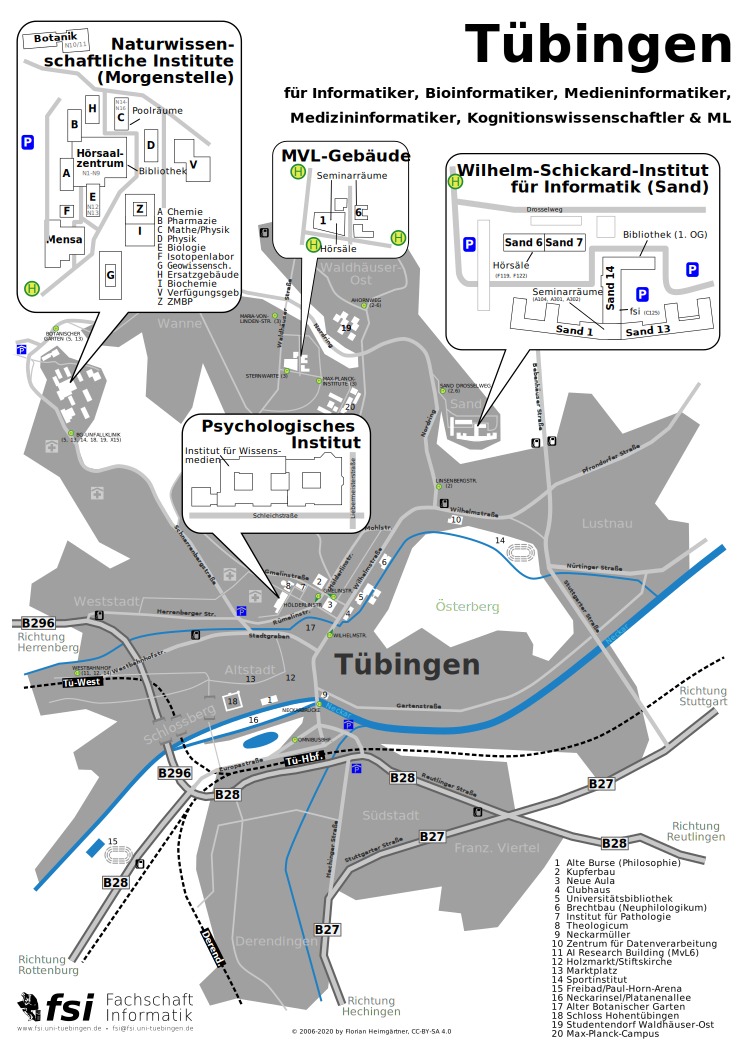
\includepdf[delta=5mm 5mm]{pdf/stadtplan.pdf}
  \end{letter}
\end{document}
